\documentclass[compress]{beamer}
\useoutertheme[footline=authorinstitutetitle]{miniframes}
\usecolortheme{whale}
\usecolortheme{orchid}
\useinnertheme{rounded}

\setbeamerfont{block title}{size={}}

%\usepackage{beamerthemeproyxetex}
%\usepackage{synttree}

\title{Introducing myself}
\author{Maarten van Gompel}
\date{October 2011}
\usepackage{graphicx}
\usepackage{placeins}



\def\raccoon{
\makebox[\linewidth][c]{\includegraphics[width=70pt]{/home/proycon/Pictures/All/raccoon.pdf}\FloatBarrier}
}
\def\smallraccoon{
\makebox[\linewidth][c]{\includegraphics[width=30pt]{/home/proycon/Pictures/All/raccoon.pdf}\FloatBarrier}
}



\begin{document}

\begin{frame}
	\titlepage
	\smallraccoon    
\end{frame}


\section{Past}

\begin{frame}

	\begin{block}{Work}
		\begin{itemize}
			\item Scientific Programmer, Tilburg University
		\end{itemize}
	\end{block}


	\begin{block}{Study}
		\begin{itemize}
			\item \textbf{Master:} Human Aspects of Information Technology, Tilburg University 
			\item \textbf{Bachelor:} Cognitive Artificial Intelligence, Utrecht University
		\end{itemize}
	\end{block}

\end{frame}


\section{Projects}


\begin{frame}

	\begin{block}{Projects / Software}
		\begin{itemize}
			\item \textbf{DutchSemCor} -- Construction of a lexical semantic sense-annotated corpus for Dutch, in part using automatic Word Sense Disambiguation  \\
			\item \textbf{PBMBMT}: Phrase based memory-based Machine Translation  \\
			\item \textbf{FoLiA}: Format for Linguistic Annotation -- Universal, extensible and highly expressive XML-based format for the representation of annotated language resources. \\
			\item \textbf{CLAM} -- Software to easily turn command-line NLP tools into fully fledged RESTful web-services (with web-application frontend).  \\
			\item \textbf{PyNLPl}: Python Natural Language Processing Library \\
			\item \textbf{ucto}: unicode tokeniser (for Dutch, English, and others). \\
			\item \textbf{Frog}: PoS-tagger/parser/lemmatiser suite (successor of Tadpole) \\
		\end{itemize}
	\end{block}
\end{frame}

\begin{frame}
	\begin{block}{Open Source}
		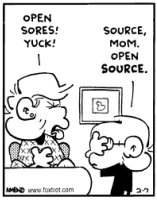
\includegraphics[width=3cm]{opensource.jpg}\FloatBarrier
	\end{block}

	\begin{block}{Github}
		http://github.com/proycon
	\end{block}
\end{frame}

\section{Interests}

%\begin{frame}

%	\begin{block}{Interests}
%		\large{\textbf{Language and Technology}}
%	\end{block}

%	\begin{block}{Interests: Language}
%		\begin{itemize}
%			\item Multilingualism/Polyglotism
%			\item (2nd) Language Acquisition
%			\item Specific languages: Portuguese, Spanish, French, Italian, Esperanto, Arabic, Russian, Chinese
%		\end{itemize}
%	\end{block}

%	\begin{block}{Interests: Technology}
%		\begin{itemize}
%			\item Linux
%			\item Python
%			\item C++
%			\item Web-application development (Django) and RESTful webservices
%			\item e-Learning
%		\end{itemize}
% \end{block}

%\end{frame}

\begin{frame}

	\begin{block}{Interests: Language Technology}
		\begin{itemize}
			\item Machine Translation
			\item Computer-aided Language Learning
			\item Machine Learning
			\item Word Sense Disambiguation
			\item Pattern finding
			\item Annotation Formats for Language Resources
			\item Searching in large corpora
		\end{itemize}
	\end{block}
\end{frame}

\section{Present \& Future: My PhD Research}

\begin{frame}

	\begin{block}{COLIBRI (1/4)}
		\textbf{My PhD Research:} \emph{Constructions as Linguistic Bridges (COLIBRI)} \\

		\textbf{First stage:} \emph{The identification and extraction of ``good'' constructions from corpus data} \\

		\textbf{What is a ``construction''}? \\
		\begin{itemize}
			\item A \emph{pattern} of words, possibly with gaps, which in some way forms an entity
			\item Constructions emerge from the data (parallel corpora) rather than linguistic theory
			\item The intuitive ``atom'' in memory-based language processing
			\item A level above n-gram models and below linguistic syntax
		\end{itemize}

	\end{block}
\end{frame}


\begin{frame}

	\begin{block}{COLIBRI (2/4)}

		\textbf{Second stage:} \emph{Establishing aligned constructions} \\

		\begin{itemize}
			\item Aligned constructions are a mapping of constructions in one language, to constructions in another language.
		\end{itemize}

	\end{block}

\end{frame}


\begin{frame}

	\begin{block}{COLIBRI (3/4)}

		\textbf{Third stage:} \emph{Local translation step -- Classification using construction-experts} \\

		\begin{itemize}
			\item Create small classifiers, each translating a particular construction in its context.
		\end{itemize}
	

	\end{block}

	\begin{block}{COLIBRI (4/4)}

		\textbf{Fourth stage:} \emph{Global translation step -- Decoding} \\

		\begin{itemize}
			\item Recombine translated constructions into coherent translations in the target language.
		\end{itemize}

	\end{block}

\end{frame}

\section{The End}

\begin{frame}

\raccoon

\begin{center}
\Large{Questions?}
\end{center}

\end{frame}



%%%%%%%%%%%%%%%%%%%%%%%%%%%%%%%%%%%%%%%%%%%%%%%%%%%%%%%%%%%%%%%%%%%%%%%%%%%%%%
Als jij




\end{document}  

